% created on 12/05/2020
% @author : ebazan
\chapter{Color image texture analysis based on Gabor features}


In this chapter we present the spectral decomposition of a color image by means of the Gabor filter. We use the theory developed in Chapter 3 about Gabor functions to extract local texture features of a color image. The main strategy consist on from transforming the input image from a three-channel real color space into a two-channel complex color representation. Then, we use a bank of Gabor filters on each channel of the image to extract the texture information generated by the variations of color and illumination in the image.

\section{Introduction}

Gabor filters have long been used for analyzing textures and extracting corresponding image features. Its adaptability and customization depending on the application and the relationship with the human visual system \cite{Daugman:JOSA:1985a}, have made this technique one of the most relevant for the analysis of textures in an image.
Some of the most recognized works in literature date back to the late 90s, where this technique was a hot research topic for image texture analysis.

The use of Gabor filters for image texture analysis is highly dependent on the final application. However, regarding the works present in the literature, we can make a clear separation taking into account the nature of the extracted features. The first group uses Gabor filters to extract a global texture descriptor (Gabor signature). Generally this strategy is suitable for applications where the images contain homogeneous textures and it is sought to make the the classification of images or an image retrieval system based on the content, as we can see in Chapter \ref{ch:distance_between_distributions}. The second group is characterized by using Gabor filters to obtain local texture features present in an image. Such a strategy is suitable for image segmentation tasks. In this chapter we address in a detailed and comprehensive way the second case, delving into the spectral decomposition of color images to obtain texture features generated by the changes in illumination and/or color.

In both aforementioned cases of use, we take advantage of the Gabor function's dual-domain (spatial and frequency) representation capability to create a bank of filters $\{g_{f, \theta}(x, y) \}$ that works at different central frequencies $f$ (scales) and orientations $\theta$ to obtain the spectral decomposition of an input image $I(x, y)$ through the convolution operation of each of the filters. 

\begin{equation}\label{eq:gabor_responses}
    r_{f, \theta}(x,y) = I(x, y) \ast g_{f, \theta}(x,y)
\end{equation}

As we know, due to the complex form of Gabor's filters \ref{eq:gabor_function_2d_spacefreq_bank} defined in the chapter \ref{ch:gabor_filter_description}, the response of the filter $r_{f,\theta} (x, y)$ will have, in the same way as the filter, a real part and an imaginary part, here denoted as $\Re{(\cdot)}$ and $\Im{(\cdot)}$, respectively.

The linear transformation of an image using Eq. \eqref{eq:gabor_responses}, produces considerable information about the textures present in the image. The efficient manipulation of this information is the basis for the extraction of appropriate (local or global) texture features. Although this manipulation is a common denominator in techniques based on signal processing, in the literature we can find various schemes to create more separable texture features. In general, these methods can be classified according to the considered output and the post-processing of the Gabor filter outputs as follows: 

\begin{enumerate}
    \item Using the amplitude of the response (magnitude or Gabor energy) \cite{Bovik.Clark.ea:TPAMI:1990}
        \begin{equation}\label{eq:gabor_magnitude}
            |r_{f, \theta}(x,y)| = \sqrt{\Re{(r_{f, \theta}(x, y))}^2 + \Im{(r_{f, \theta}(x, y))}^2}
        \end{equation}
    \item Using the phase of the response \cite{Palm.Lehmann:MGV:2002}
    \begin{equation}\label{eq:gabor_phase}
            \arg(r_{f, \theta}(x,y)) = \arctan2{\left(\frac{\Im{(r_{f, \theta}(x, y))}}{\Re{(r_{f, \theta}(x, y))}}\right)}
        \end{equation}
    \item Using only the real component of the response \cite{Jain.Farrokhnia:IJPR:1991}
    \begin{equation}\label{eq:gabor_real_part}
            \Re{(r_{f, \theta}(x, y))}
        \end{equation}
    \item Using the square amplitude of the response (Gabor local power spectrum) \cite{Grigorescu.Petkov.ea:TIP:2002}
    \begin{equation}\label{eq:gabor_power}
            |r_{f, \theta}(x,y)|^2 = \Re{(r_{f, \theta}(x, y))}^2 + \Im{(r_{f, \theta}(x, y))}^2
        \end{equation}
\end{enumerate}

After selecting the type of output, the most common post-processing of the Gabor filter outputs in the literature consists of applying a non-linear transformation followed by smoothing using a rectangular or Gaussian window \cite{Randen.Husoy:TPAMI:1999}, \cite{Clausi.EdJernigan:JPR:2000}. The application of non-linearity favors the activation of the textured areas in the images, while the smoothing favors the location of the energy obtained with the filter, avoiding the loss of information from the natural contours of the image. Figure \ref{fig:general_pipeline_gabor_feature_extraction} illustrate the aforementioned scheme showing the possible steps (boxes with black continuous lining) and the posible input/outpus (boxes with black dotted lining) we can use to extract texture feaures from images.

\begin{figure}
\centering
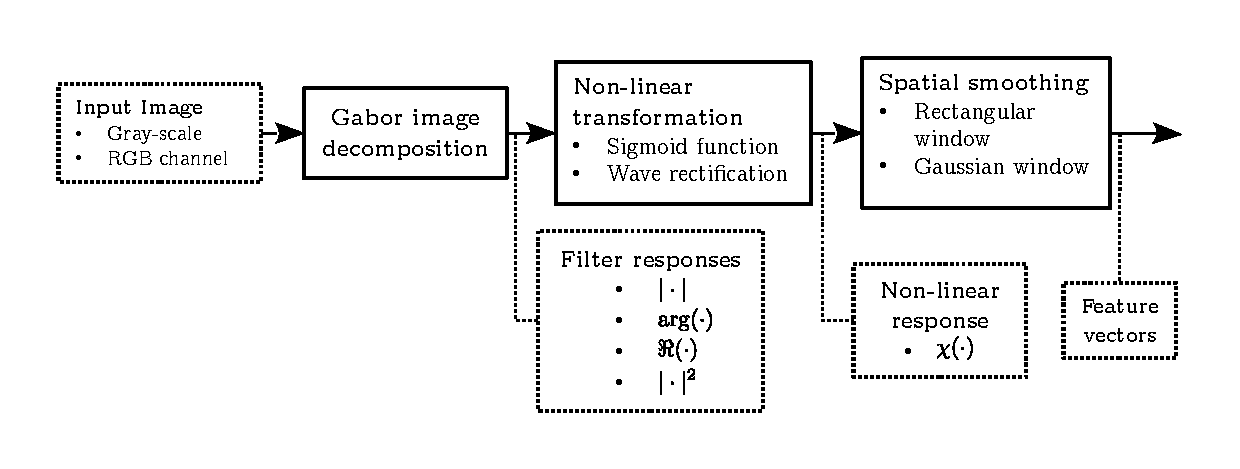
\includegraphics{texture_feature_extraction_pipeline.pdf}
\caption{General pipeline for extraction of texture features using the Gabor filters}\label{fig:general_pipeline_gabor_feature_extraction}
\end{figure}

\subsection{Color Gabor features}

There are several techniques to obtain texture features from color images. The simplest and most direct is to transform the color image into a grayscale image. This strategy allows reducing the number of channels in the image to subsequently apply the pipeline of Fig. \ref{fig:general_pipeline_gabor_feature_extraction}. For example, for an image in the RGB color space, the grayscale image represents the levels of red, green, and blue at a single luminance value from which we can extract texture features corresponding to lighting variation. However, despite the good results in images with homogeneous grayscale textures, reducing channels for a natural color image with non-homogeneous textures does not ensure the generation of representative texture features. This is because the non-homogeneous textures in a color image are not only generated by lighting variations,  but also by variations in chromaticity, therefore, the gray-scale image transformation leads to a minimization, or lost in the worst case, of textures generated by the color changes.


\textit{Idea to develope:} Illustrate the effect of compute unichrome features in the gray-scale and the RGB space for a color image.

One way to avoid the post-processing stage is to first transform the color image in a color space that handles the coupling between the color channels rather than separating them as components of the color space, and then performing the Gabor decomposition. One possible option for the color representation is the quaternion framework \cite{Sangwine.Ell: VISP: 2000}. This encodes the color value of each pixel in a pure quaternion, where the real component is set to zero and the three imaginary components represent the color band such as $I(x, y) = R (x, y) i + G (x, y) j + B (x, y) k $. This 3-component vector representation yields a system which has well-defined mathematical operations, such as Quaternion Fourier Transform, which makes possible the Gabor image decomposition by means of the Quaternion Gabor Filters (QBF) \cite{Subakan.Vemuri:EMMCVPR:2009}. However, when using quaternion values, the non-existing commutativity has to be taken into account, in addition, the QGF does not support any physic interpretation of what is measured.

\section{Two-channel complex image representation}

We can have the color information obtained to build a two channel image that contains pure luminance values in one channel and complex chrominance values in the other channel through the transformation from the RGB to the HLS/HSV or $Lab$ color spaces. The complex value can be defined depending upon the two chrominance variables $H$ and $S$ in the case of $HLS$ or by using $a$ and $b$ in case of $Lab$ color space. 

We define the combined chrominance exponential for HSV as

\begin{equation}\label{eq:chrominance_hsv}
    Chr(x,y) = S(x,y) e^{iH(x,y)}
\end{equation}

where H is the hue and S is the saturation value obtained after the RGB to HLS transformation. While combined chrominance function for $Lab$ is defined as:

\begin{equation}\label{eq:chrominance_lab}
    Chr(x,y) = a + jb
\end{equation}
where $a$ and $b$ are two chroma variables obtained from RGB to $Lab$ transformation. We obtain a complex representation of chrominance content of the image whose spectrum is interesting to analyze in order to characterize the spatial variations of the chromatic part of the image. 


